\documentclass{article}

\usepackage[spanish]{babel}
\usepackage[utf8]{inputenc}
\usepackage[T1]{fontenc} % allows to copy accented words on PDF
\usepackage{blindtext}
\usepackage[letterpaper, margin=1in]{geometry}
\usepackage{url}
\usepackage{pgfplots}
\pgfplotsset{width=10cm,compat=1.9}
\usepackage{graphicx}
\usepackage{booktabs}
\usepackage{amsmath}
\usepackage{listings}
\usepackage{lmodern}
\usepackage[framed,numbered,captionpos=t]{matlab-prettifier}
\usepackage{color} %red, green, blue, yellow, cyan, magenta, black, white
\usepackage{xcolor} %for coding
\usepackage{tikz}

\definecolor{gray97}{gray}{.97}
\definecolor{gray75}{gray}{.75}
\definecolor{gray45}{gray}{.45}
\definecolor{mygreen}{RGB}{28,172,0} % color values Red, Green, Blue
\definecolor{mylilas}{RGB}{170,55,241}
%----Java----
\definecolor{mygreen}{rgb}{0,0.6,0}
\definecolor{mygray}{rgb}{0.5,0.5,0.5}
\definecolor{mymauve}{rgb}{0.58,0,0.82}

\lstset{ %
  backgroundcolor=\color{white},   % choose the background color
  style      = Matlab-editor,
  basicstyle = \mlttfamily,
  numbers=left,
  stepnumber=1,
  xleftmargin=.1\textwidth,
  xrightmargin=.1\textwidth,
  %basicstyle=\footnotesize,        % size of fonts used for the code
  breaklines=true,                 % automatic line breaking only at whitespace
  captionpos=t,                    % sets the caption-position to bottom
  commentstyle=\color{mygreen},    % comment style
  escapeinside={\%*}{*)},          % if you want to add LaTeX within your code
  keywordstyle=\color{blue},       % keyword style
  stringstyle=\color{mymauve},     % string literal style
  morekeywords={run, getDimensions, newArray, getResult}
}

% Código
\definecolor{codegreen}{rgb}{0,0.6,0}
\definecolor{codegray}{rgb}{0.5,0.5,0.5}
\definecolor{codepurple}{rgb}{0.58,0,0.82}
\definecolor{backcolour}{rgb}{0.95,0.95,0.92}

\lstdefinestyle{mystyle}{
	backgroundcolor=\color{backcolour},   
	commentstyle=\color{codegreen},
	keywordstyle=\color{magenta},
	numberstyle=\tiny\color{codegray},
	stringstyle=\color{codepurple},
	basicstyle=\ttfamily\footnotesize,
	breakatwhitespace=false,         
	breaklines=true,                 
	captionpos=b,                    
	keepspaces=true,                 
	numbers=left,                    
	numbersep=5pt,                  
	showspaces=false,                
	showstringspaces=false,
	showtabs=false,                  
	tabsize=2
}

\lstset{style=mystyle}

% Cabecera y pie de página
\usepackage{fancyhdr}
\pagestyle{fancy}
\fancyhf{}
\rhead{Práctica 1: Nombre de la práctica}
\lhead{Instituto Tecnológico de Oaxaca}
\cfoot{\thepage}
% -=-=-=-=-=-=-=-=-=-=

% Defniciones para título y autores.............................................
\makeatletter
\def\HUGE{\@setfontsize\HUGE{24}{36}}
\def\LARGE{\@setfontsize\LARGE{18}{27}}
\def\large{\@setfontsize\large{14}{21}}
\setlength{\parskip}{0.1in}

\newcommand{\myAsignature}{ASIGNATURA}
\newcommand{\myClave}{ABC234}
\newcommand{\descripcion}{Ejercicio 0}
\newcommand{\myActivity}{DESCRIPCIÓN DE ACTIVIDAD}
\newcommand{\authora}{Martínez Mendoza Jesús Ángel}
%\newcommand{\authorb}{}
%\newcommand{\authorc}{}
%\newcommand{\authord}{}
\newcommand{\myGroup}{5SA}
\newcommand{\myControlNumber}{22161152}
\newcommand{\myReviewers}{Leonardo Leo Donatelo Rafael}
\newcommand{\myPeriod}{AGO - DIC /2025}
\newcommand{\myDate}{Oaxaca de Juárez, Oax, 31 jul 2024}
%...............................................................................

\begin{document}

% archivo de la portada
\begin{titlepage}

    \begin{tikzpicture}[remember picture, overlay]
        % Dibujar las dos líneas verticales en el lado izquierdo y menos largas
        \draw[thick] (current page.north west) ++(1cm,-2cm) -- ++(0,-24cm);
        \draw[thick] (current page.north west) ++(1.2cm,-2cm) -- ++(0,-24cm);
    \end{tikzpicture}
    
    \begin{center}
    %\vspace{0.2in}
    
\includegraphics[width=0.3\textwidth]{images/logo-tecnm}\hspace{0.3in}
    
\includegraphics[width=0.15\textwidth]{images/logo-ito}\hspace{0.3in}
    
\includegraphics[width=0.25\textwidth]{images/logo-sep}
    
    \rule[1cm]{\textwidth}{3pt}
    
    %Encabezado-------------------------------------------------------------------
    \vspace{-1cm}
    {\Large
    \textbf{TECNOLÓGICO NACIONAL DE MÉXICO}\\[0.5cm]
	\LARGE
    \textbf{INSTITUTO TECNOLÓGICO DE OAXACA}\\[0.5cm]
	\normalsize
	\textbf{\textit{"Tecnología Propia e Independencia Económica"}}
	}
	
    %Asignatura-----------------------------------------------------------------
    \vspace{1cm}
    \LARGE
    \underline{\textbf{\myAsignature}} \\
    \small
    \myClave

    %Carrera---------------------------------------------------------------------
    \vspace{1cm}
    \large
    Carrera: \textbf{INGENIERÍA EN SISTEMAS COMPUTACIONALES}
    
    %Actividad-------------------------------------------------------------------
    \vspace{1cm}
    {\large
    Actividad: \descripcion \\
    \textbf{"\myActivity"}\\[0.5cm]
    }
    \vspace{0.5cm}
    
    %Datos del alumno------------------------------------------------------------
    \begin{flushleft}
    {\large
		 Presenta:\\    
			\textbf{\authora}\\
            %\textbf{\authorb}\\
            %\textbf{\authorc}\\
            %\textbf{\authord}\\
            Grupo: \textbf{\myGroup} | Matrícula: \textbf{\myControlNumber}
	}
    \end{flushleft}

    
    %Datos del docente-----------------------------------------------------------
    \begin{flushright}
    {\Large
        Docente:
        
    		\textbf{\myReviewers}
		}
    \end{flushright}
    \vfill
    
    %Fecha-----------------------------------------------------------------------
    {\large Periodo: \myPeriod}\\
    \vspace{0.5cm}
    {\large \myDate}
    
    \end{center}
\end{titlepage}

% índice de contenido
\tableofcontents

\newpage

\section{Introducción}

% Considere que las referencias están en formato \textit{Bibitems} y se incluyen al final de este archivo.

Este es un ejemplo de como se deben insertar referencia en el documento~\cite{conagua-2011}. Considere que las referencias están en formato \textit{Bibitems} y se incluyen al final de este archivo~\cite{conagua-2011,undesa2008}.


% Texto dummy para rellenar el documento
\blindtext[2]

 % ejemplo de figura
\begin{figure}[htb]
    \centering
    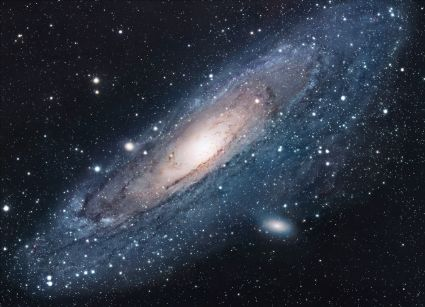
\includegraphics[width=3.5in]{images/universe}
    \caption{Pie de texto en la figura.}
    \label{fig:universe}
\end{figure}

\blindtext[3]
\section{Objetivos}

\subsection{Objetivo general}
\blindtext[1]

\subsection{Objetivos específicos}

\begin{itemize}
	\item Primer elemento y su descripción relacionada con los objetivos.
	\item Segundo elemento y su descripción relacionada con los objetivos.
	\item Tercer elemento y su descripción relacionada con los objetivos.
	\item Cuarto elemento y su descripción relacionada con los objetivos.
\end{itemize}

\section{Marco Teórico}

\blindtext[2]

El Error Cuadrático medio queda definido por la Ecuación \eqref{eq:mse}:

\begin{equation}
	MSE(X,h_\theta)=\frac{1}{m}\sum_{i=0}^m\left(\theta x^{(i)}-y^{(i)} \right)^2 \label{eq:mse}
\end{equation}

\section{Desarrollo}

\blindtext[1] \\
Este es un ejemplo de una cita \cite{Sarker2014} \\
Este es otro ejemplo de una cita \citet{Topley2010} \\
Este es otro ejemplo de una cita \citep{Sarker2014} \\

Código en Python
\lstinputlisting[language=Python, caption={Código de Ejemplo en Python}, label={lst:example}]{codigo/python.py}

\section{Resultados}

\blindtext[1]

Plotting from data:

\begin{figure}[htb]
\centering
\begin{tikzpicture}
\begin{axis}
[
	title={Resultados de la medición},
	xlabel={$x$ Temperature [\textcelsius]},
  ylabel={Solubility [g per 100 g water]},
    xmin=0, xmax=100,
    ymin=0, ymax=120,
    xtick={0,20,40,60,80,100},
    ytick={0,20,40,60,80,100,120},
    legend pos=north west,
    ymajorgrids=true,
    grid style=dashed
]

\addplot[
    color=blue,
    mark=square,
    ]
    coordinates {
    (0,23.1)
    (10,27.5)
    (20,32)
    (30,37.8)
    (40,44.6)
    (60,61.8)
    (80,83.8)
    (100,114)
    };
    \legend{Data $f(x)$}
\end{axis}
\end{tikzpicture}
\end{figure}

\section{Bibliografía y Citas}

\printbibliography


\end{document}
